\section{Definitionen \& Formate}
Beschreibung der wichtigsten Codex und Datei-Formate, die während des Projektes zum Einsatz kamen.

%%%%%%%%%%%%%%%%%%%%%%%%%%%%%%%%%%%%%%%%%%%%%%%%%%%%%%%%%%%%%%%%%%%%%%%%%%%%%%%
\subsection{webm}
Wurde als Alternative zu H.264 von Google 2010 entwickelt und 2011 von Google auf YouTube eingeführt. Es kann auf Html5 Webseiten ohne Browserplugin Video und Audio streamen. Es verwendet für die Videokodierung VP8 oder VP9 und für Audio Vorbis oder Opus. Das WebM Format löst damit den Flashplayer ab.\\

Html5 Snippet von www.w3Schools.com zur Anzeige von webm.
\begin{verbatim}
<video width="320" height="240" controls>
  <source src="movie.webm" type="video/webm">
  Your browser does not support the video tag.
</video> 
\end{verbatim}

%%%%%%%%%%%%%%%%%%%%%%%%%%%%%%%%%%%%%%%%%%%%%%%%%%%%%%%%%%%%%%%%%%%%%%%%%%%%%%%
\subsection{h264}
H.264 ist ein Standard zur Kompression von Videodaten. Bei der Komprimierung in dieses Format werden viele Algorithmen verwendet und es erfordert hohe Hardwareanforderungen, verglichen mit anderen Komprimierungsverfahren. Häufig werden die Berechnungen mit Hardwareunterstützung auf den Computational Units der Grafikkarte ausgeführt. Ein wichtiges Feature des H.264 Kodex ist der Abgleich mit einem gespeicherten Frame. Es wird der Unterschied (Motion Estimation) berechnet und nur die Differenz an den Klienten gesendet. Die Frequenz mit der ein Basisframe (vollständiges Bild) gesendet wird ist bei gstreamer einstellbar.\\

\begin{minipage}{\textwidth}
    \begin{center}
        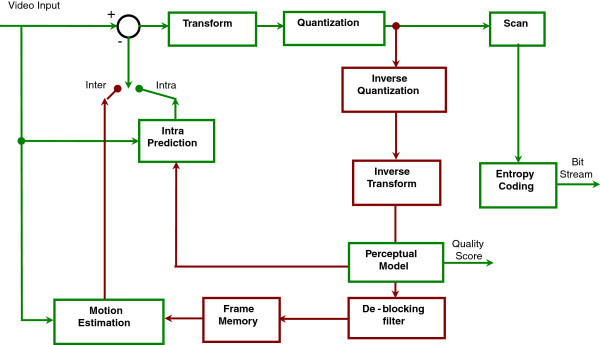
\includegraphics[scale=4.0]{img/h264.jpg} 
    \end{center}
\end{minipage}
\begin{center}
Schemaplan H.264
\end{center}

\section{Vergleich der Streaming-Lösungen und Tests} \label{RefVergleich}
Die Ergebnisse der Versuche wurden übersichtlich in Tabelle 1 zusammengefasst. Von den Ergebnissen ausgehend, wurde die gstreamer Bibliothek für das Streaming vom emb. System ausgewählt und ffmpeg für das zurückstreamen. Gstreamer schien ungeeignet für das zurückstreamen zu sein, da die CPU Leistung des emb. Systems nicht ausreichte, um die Frames auszupacken. Selbst unkomprimierte RAW Frames konnten nicht die Anforderung erfüllen, siehe gstreamer Kapitel \ref{RefGstreamer}.

\begin{table}[H]
\centering
 \begin{tabular}{l|c|c|c}
 \textbf{Streamingtest}&\textbf{Audiodelay [s]}&\textbf{Videodelay [s]} & \textbf{CPU [\%]}\\
\cline{1-4} 
 (a) Testaudio gstreamer PC > localhost          & instant   & --    & --\\
 (b) Testaudio gstreamer emb. System > localhost & instant   & --    & emb.3\\
 (c) Testbild gstreamer PC > localhost           & --        & instant & --\\
 (d) Testbild gstreamer emb. System > localhost  & --        & instant & emb.20\\                        
 (e) Audio gstreamer PC > localhost              & instant   & --    & --\\
 (f) Audio gstreamer emb. System > localhost     & instant   & --    & --\\
 (g) Video gstreamer PC > localhost              & --        & 0.1   & --\\
 (h) A/V gstreamer emb.Sys > PC                  & 0.1       & 0.1   & emb.30\\
 (i) A/V gstreamer PC > emb.System               & ? 20+     & ? 20+ & emb.100\\ 
 \cline{1-4}
 (j) Audio PC ffmpeg > ffplay (localhost)            & 0.2   & --   & --\\
 (k) Audio PC ffmpeg > ffserver > ffplay (localhost) & 0.4   & --   & --\\
 (l) Video PC ffmpeg > ffserver > ffplay (localhost) & --    & 1.4  & --\\
 (m) A/V emb.Sys.ffmpeg > PC ffserver > PC ffplay    & >2.5  & >2.5 & emb.30\\
 (n) A/V PC ffmpeg > PC ffserver > emb.Sys. ffplay   & >1.5  & >1.5 & emb.100\\
\end{tabular}

     \caption{Streaming Delayzeiten}
     \label{tbl:beispieltabelle}
     % Verweis im Text mittels \ref{tbl:beispieltabelle}
   \end{table}

%%%%%%%%%%%%%%%%%%%%%%%%%%%%%%%%%%%%%%%%%%%%%%%%%%%%%%%%%%%%%%%%%%%%%%%%%%%%%%%
\newpage
\section{Anhang: Werbeblatt Jolandi Workerbot4} \label{RefAnhang}
Werbeprospekt für den Service Roboter Jolandi auf zwei Seiten.\\

   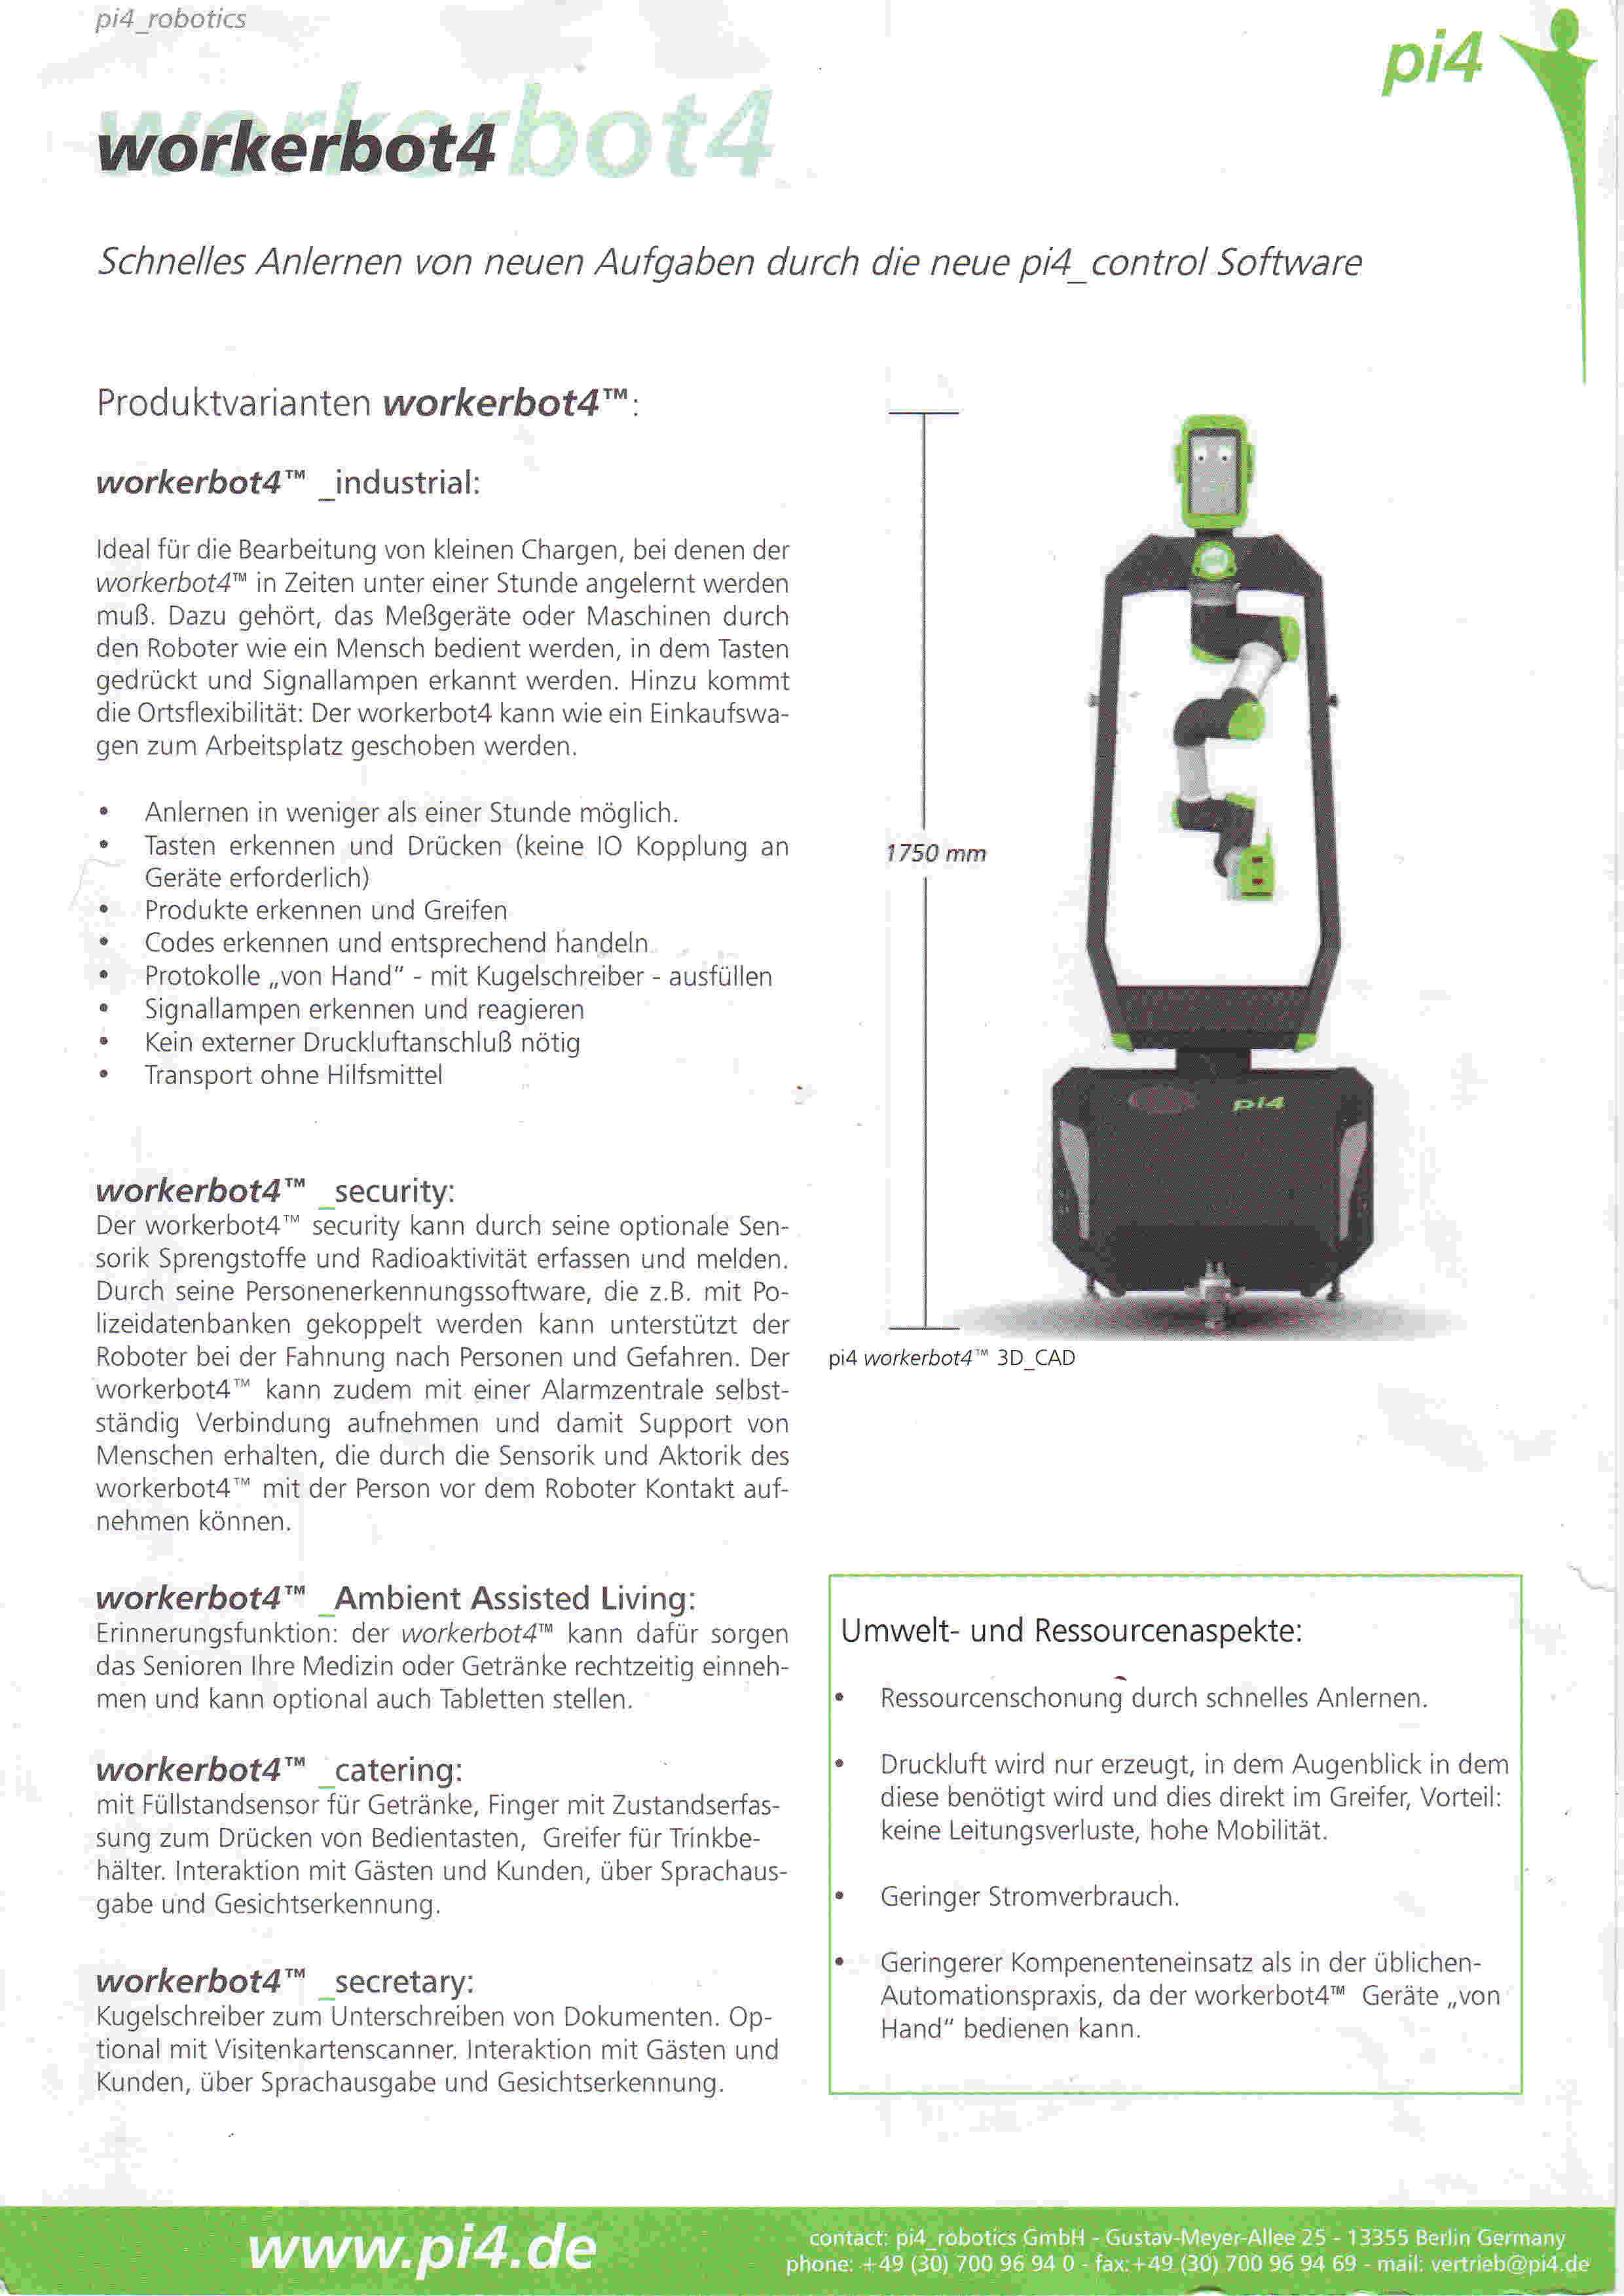
\includegraphics[scale=0.75]{img/jolandi1.jpg} 
   
   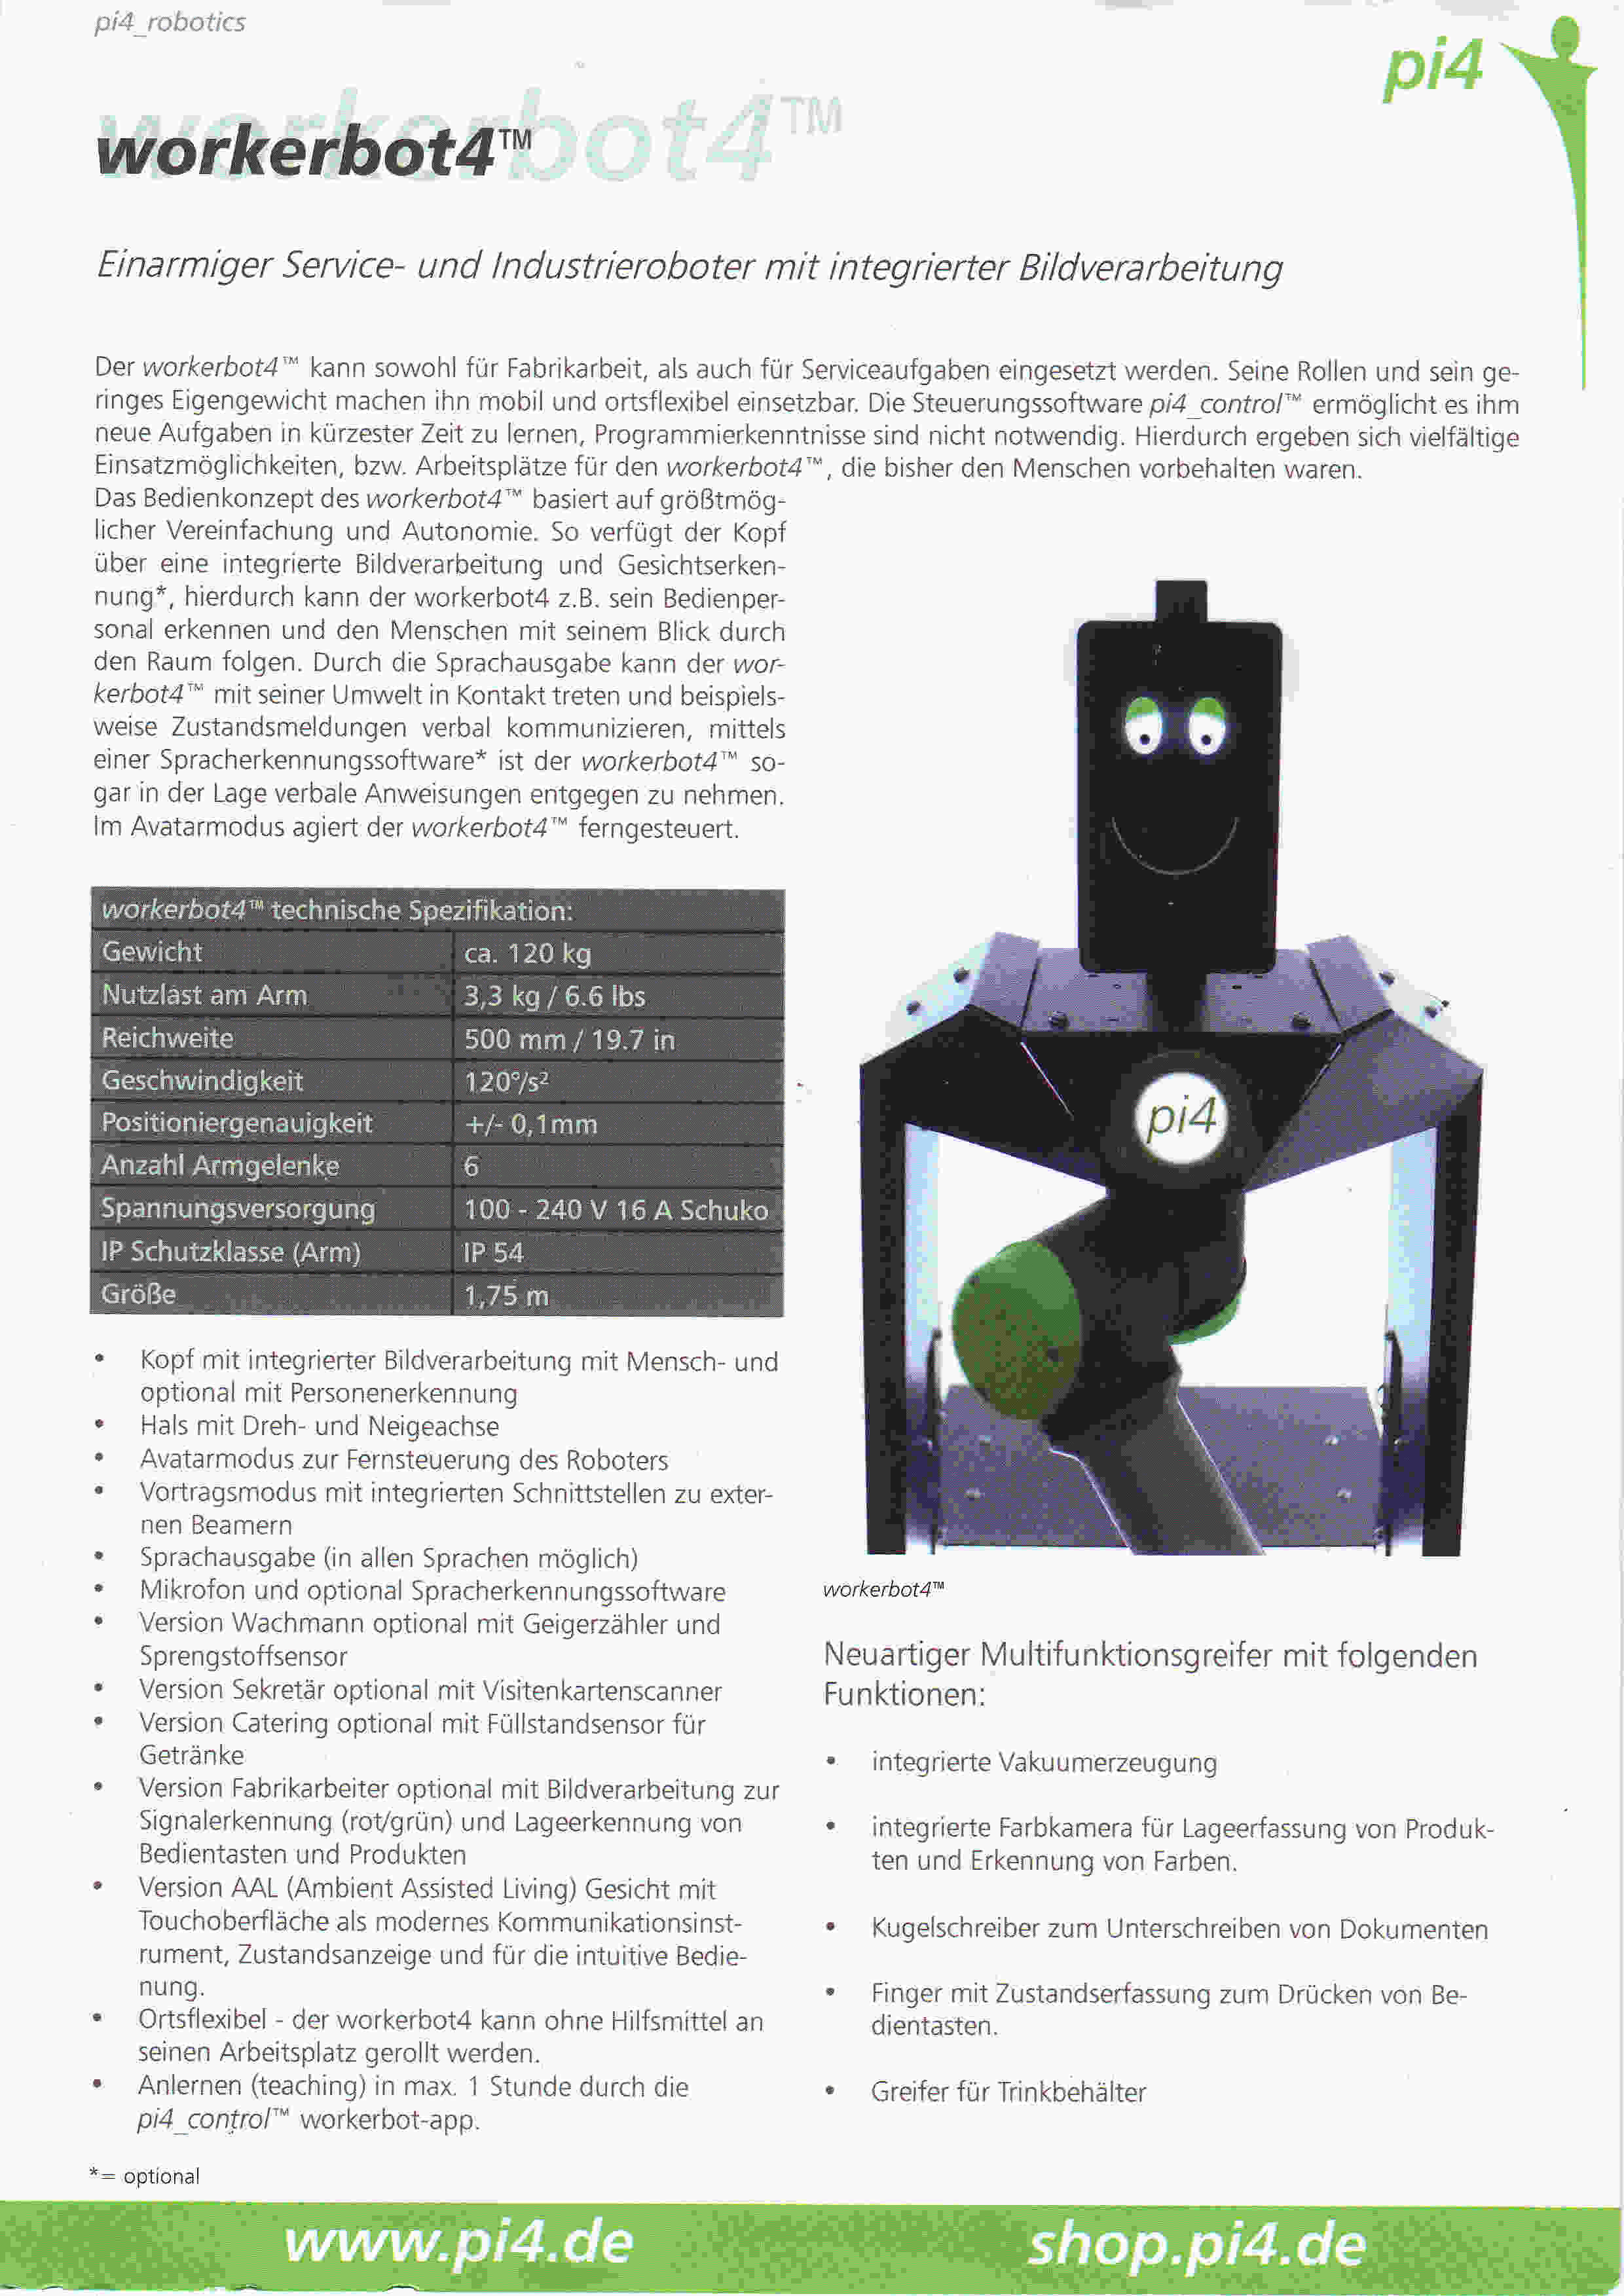
\includegraphics[scale=0.75]{img/jolandi2.jpg} 


